\begin{frame}{EPR}{}
\begin{columns}[c,onlytextwidth]
\begin{column}{0.51\textwidth}
\begin{figure}
	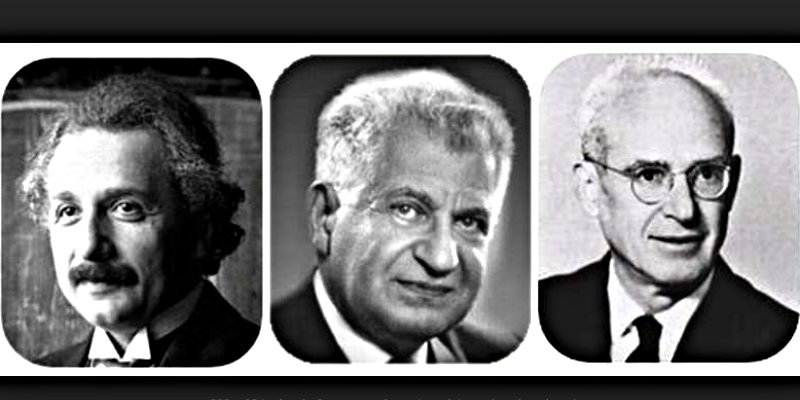
\includegraphics[width=\linewidth]{Feathergraphics/epr}
	\caption{Albert Einstein (izquierda), Boris Podolsky (en medio) y Nathan Rosen (derecha).}
\end{figure}
\end{column}

\begin{column}{0.45\textwidth}
	En 1935, EPR plantearon la pregunta:\vspace{3mm}
	
	¿Es completa la descripción que da la teoría de la Mecánica Cuántica?
\end{column}
\end{columns}
\end{frame}


\begin{frame}{EPR}{”Definiciones:”}
\begin{itemize}
	\item \textbf{Completitud:} cada elemento de la realidad física debe tener una contraparte en la teoría física.\vspace{4mm}
	\item \textbf{Realidad:} si, sin perturbar en absoluto el sistema, podemos predecir con certeza (i.e., probabilidad igual a $1$) el valor de una magnitud física, entonces existe un elemento de la realidad física correspondiente a dicha magnitud.
\end{itemize}
\end{frame}



\begin{frame}{EPR}{Estado singlete}
Retomemos el argumento EPR mediante su reformulación con dos partículas de espín $\frac{1}{2}$, preparadas en el estado singlete:
$$ |\psi\rangle_{12} = \frac{1}{\sqrt{2}} ( |\uparrow_z\rangle_1 |\downarrow_z\rangle_2 - |\downarrow_z\rangle_1 |\uparrow_z\rangle_2 ). $$
	
	\begin{center}
		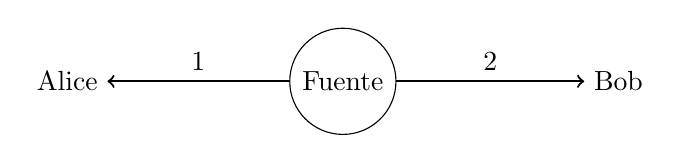
\begin{tikzpicture}
			\node (f) at (0,0) [draw,circle] {Fuente};
			\node (a) at (-3.5,0) {Alice};
			\node (b) at (3.5,0) {Bob};
			\draw[->,thick] (f) -- node[above] {1} (a);
			\draw[->,thick] (f) -- node[above] {2} (b);
		\end{tikzpicture}
	\end{center}
	
	\begin{itemize}
		\item El estado singlete es un estado entrelazado de espín total cero.
		\item Si ambos observadores miden en la misma dirección, sus resultados están perfectamente anticorrelacionados.
	\end{itemize}
\end{frame}



\begin{frame}{EPR}{Mediciones de Alice y Bob}
\textbf{(i)} Alice elige medir una componente del espín de su partícula, por ejemplo $S_z^{(1)}$.
\begin{gather*}
	\text{Si Alice mide } S_z^{(1)} = +\frac{\hbar}{2} \Rightarrow \text{el estado de Bob es } |\downarrow_z\rangle_2
	\\
	\text{Si Alice mide } S_z^{(1)} = -\frac{\hbar}{2} \Rightarrow \text{el estado de Bob es } |\uparrow_z\rangle_2.
\end{gather*}\vspace{2mm}

\textbf{(ii)} Alternativamente, Alice puede elegir medir otra componente, por ejemplo $S_x^{(1)}$.
\begin{gather*}
	\text{Si Alice mide } S_x^{(1)} = +\frac{\hbar}{2} \Rightarrow \text{el estado de Bob es } |\downarrow_x\rangle_2
	\\
	\text{Si Alice mide } S_x^{(1)} = -\frac{\hbar}{2} \Rightarrow \text{el estado de Bob es } |\uparrow_x\rangle_2.
\end{gather*}	
\end{frame}



\begin{frame}{EPR}{}
	
	\textbf{(iii)} Los operadores correspondientes a las componentes $x$ y $z$ del espín de Bob no conmutan:
	\begin{equation}
		[S_x^{(2)},S_z^{(2)}] = -i\hbar S_y^{(2)} \neq 0.
		\label{eq:contradiccion}
	\end{equation}
	
	\begin{itemize}
		\item Supongamos que la medición de Alice no perturba físicamente a la partícula distante de Bob (localidad).
		\item Como Alice puede predecir con certeza cualquiera de las dos componentes, bajo el criterio de realidad de EPR ambas deberían corresponder a elementos de realidad física.
		\item Sin embargo, no existe un estado cuántico en el que ambas componentes tengan simultáneamente valores definidos.
	\end{itemize}
	
	\begin{block}{Conclusión de EPR}
		Bajo estas suposiciones, la descripción proporcionada por la función de onda es incompleta.
	\end{block}
	
\end{frame}


%%%%%%%%%%%%%%%%%%%%%%%%%%%%%%%%%%%%%%%%
%%%%%%%%%%%%%%%%%%%%%%%%%%%%%%%%%%%%%%%%


\begin{frame}{Desigualdad de Bell}{Realismo local}
	
	Consideremos las siguientes suposiciones:
	
	\begin{itemize}
		\item \textbf{Realismo:} las variables ocultas $\lambda$, junto con las direcciones de medición, determinan los resultados de las posibles mediciones de Alice y Bob.
		\item \textbf{Localidad:} para un mismo valor de $\lambda$, el resultado de Alice no depende de la elección de Bob, y viceversa.
		\item \textbf{Independencia:} las elecciones de las direcciones de medición son estadísticamente independientes de $\lambda$.
	\end{itemize}
	
	\begin{gather*}
		A(a,b,\lambda)=A(a,c,\lambda)=A(a,\lambda),
		\\
		B(b,a,\lambda)=B(b,c,\lambda)=B(b,\lambda).
	\end{gather*}
	
	En adelante, omitiremos la dependencia en $\lambda$. Los resultados $A,B=\pm1$ corresponden a las componentes del espín en unidades de $\frac{\hbar}{2}$.
	
\end{frame}


\begin{frame}{Desigualdad de Bell}{Representación gráfica}
	\begin{columns}[c,onlytextwidth]
		\begin{column}{0.46\textwidth}
			\begin{figure}
				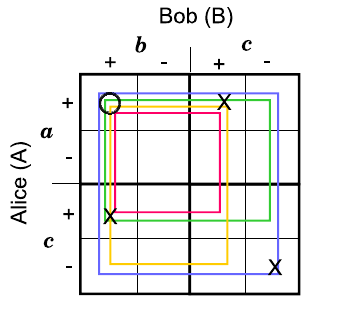
\includegraphics[width=\linewidth,height=0.55\textheight,keepaspectratio]{Feathergraphics/grafica}
				\caption{Representación de R\k{e}bilas.}
				\label{fig:graf}
			\end{figure}
		\end{column}
		
		\begin{column}{0.51\textwidth}
			\small
			\begin{itemize}
				\item Alice puede elegir medir en las direcciones $a$ o $c$, mientras que Bob puede elegir entre $b$ o $c$.
				\item Cada par de partículas tiene resultados asignados para las cuatro combinaciones posibles de medición.
				\item Cada rectángulo representa una posible asignación de resultados, cuyos vértices corresponden a dichas combinaciones.
			\end{itemize}
		\end{column}
	\end{columns}
	
	Para reproducir las anticorrelaciones perfectas del estado singlete, el modelo debe satisfacer
	$$ A(c)=-B(c). $$
	
\end{frame}


\begin{frame}{Desigualdad de Bell}{}
\begin{columns}[c,onlytextwidth]
\begin{column}{0.38\textwidth}
	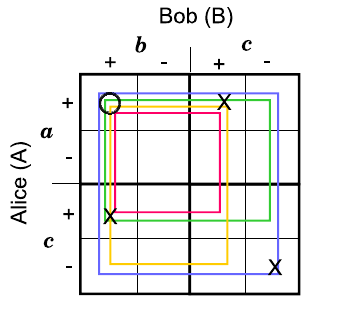
\includegraphics[width=\linewidth]{Feathergraphics/grafica}
\end{column}

\begin{column}{0.59\textwidth}
	\small
	Consideremos el conjunto de pares de partículas que producirían los resultados $A(a)=+1$ y $B(b)=+1$, denotado por $\{a^+,b^+\}$.
	\vspace{2mm}

	Dado que $A(c)=-B(c)$, la posibilidad $\{c^-,c^-\}$ queda excluida. Por lo tanto, todo par que pertenezca a $\{a^+,b^+\}$ debe pertenecer también a $\{a^+,c^+\}$ o a $\{c^+,b^+\}$.
\end{column}
\end{columns}

\vspace{2mm}
Si $n(a^+,b^+)$ representa el número de pares de partículas que producirían los resultados $\{a^+,b^+\}$, entonces
\begin{equation}
	n(a^+,b^+) \leq n(a^+,c^+) + n(c^+,b^+).
	\label{eq:des_1}
\end{equation}
\end{frame}


\begin{frame}{Desigualdad de Bell}{}
De manera análoga, intercambiando los signos,
\begin{equation}
	n(a^-,b^-) \leq n(a^-,c^-) + n(c^-,b^-).
	\label{eq:des_2}
\end{equation}

Sumando las Ecuaciones \ref{eq:des_1} y \ref{eq:des_2},
\begin{align*}
	n(a^+,b^+)+n(a^-,b^-)
	\leq& n(a^+,c^+)+n(a^-,c^-)	\\
	&+n(c^+,b^+)+n(c^-,b^-).
\end{align*}

Definimos $n_{=}(a,b)=n(a^+,b^+)+n(a^-,b^-)$.
\begin{equation}
	n_{=}(a,b)\leq n_{=}(a,c)+n_{=}(c,b).
	\label{eq:des_4}
\end{equation}
\end{frame}


\begin{frame}{Desigualdad de Bell}{}
Considerando también mediciones en las direcciones comunes $b$ y $c$,
\begin{gather*}
	A(b)=-B(b),	\\
	A(c)=-B(c).
\end{gather*}
Por lo tanto,
$$ A(c)=B(b) \Leftrightarrow A(b)=B(c), $$
lo que implica que $n_{=}(c,b)=n_{=}(b,c)$.
	
Sustituyendo en la Ecuación \ref{eq:des_4} y reorganizando,
\begin{equation}
	n_{=}(a,b)-n_{=}(a,c)\leq n_{=}(b,c).
	\label{eq:des_5}
\end{equation}
\end{frame}


\begin{frame}{Desigualdad de Bell}{}
Repitiendo el procedimiento gráfico, pero intercambiando las direcciones $b$ y $c$,
\begin{gather*}
	n(a^+,c^+) \leq n(a^+,b^+) + n(b^+,c^+),\\
	n(a^-,c^-) \leq n(a^-,b^-) + n(b^-,c^-).
\end{gather*}

Sumando ambas expresiones y utilizando la definición de $n_{=}$,
\begin{equation}
	n_{=}(a,c)-n_{=}(a,b)\leq n_{=}(b,c).
	\label{eq:des_6}
\end{equation}

Combinando las Ecuaciones \ref{eq:des_5} y \ref{eq:des_6},
\begin{equation}
	|n_{=}(a,b)-n_{=}(a,c)|\leq n_{=}(b,c).
	\label{eq:des_7}
\end{equation}
\end{frame}


\begin{frame}{Desigualdad de Bell}{Probabilidad de obtener resultados iguales}
Consideremos un conjunto de $N$ pares de partículas preparados bajo las mismas condiciones.
$$ P_{=}(a,b)=\frac{n_{=}(a,b)}{N}, $$
donde $P_{=}(a,b)$ representa la probabilidad de obtener resultados iguales al medir en las direcciones $a$ y $b$ (en el límite estadístico).
	
Dividiendo la Ecuación \ref{eq:des_7} entre $N$,
\begin{equation}
	|P_{=}(a,b)-P_{=}(a,c)|\leq P_{=}(b,c).
	\label{eq:des_proba}
\end{equation}
\end{frame}


\begin{frame}{Desigualdad de Bell}{Función de correlación}
La correlación es el valor esperado del producto de los resultados de Alice y Bob:
$$ C(a,b)=\langle A(a)B(b)\rangle. $$
\begin{center}
\begin{tabular}{c c c}
	\hline
	$A$ & $B$ & $AB$ \\
	\hline
	$+1$ & $+1$ & $+1$ \\
	$-1$ & $-1$ & $+1$ \\
	$+1$ & $-1$ & $-1$ \\
	$-1$ & $+1$ & $-1$ \\
	\hline
\end{tabular}
\end{center}

\begin{equation}
	C(a,b)=P_{=}(a,b)-P_{\neq}(a,b).
	\label{eq:correlacion}
\end{equation}
\end{frame}


\begin{frame}{Desigualdad de Bell}{Correlación y probabilidad}
Debido a que los resultados solamente pueden ser iguales o diferentes,
\begin{align*}
	P_{=}(a,b)+P_{\neq}(a,b)=&1	\\
	P_{\neq}(a,b)=&1-P_{=}(a,b).
\end{align*}

Sustituyendo en la Ecuación \ref{eq:correlacion},
\begin{align*}
	C(a,b)&=P_{=}(a,b)-[1-P_{=}(a,b)]\\
	&=2P_{=}(a,b)-1.
\end{align*}

Finalmente,
\begin{equation}
	P_{=}(a,b)=\frac{1+C(a,b)}{2}.
	\label{eq:correlacion_probabilidad}
\end{equation}
\end{frame}


\begin{frame}{Desigualdad de Bell}{}
Sustituyendo la Ecuación \ref{eq:correlacion_probabilidad} en la Ecuación \ref{eq:des_proba},

\begin{align*}
	\left|\frac{1+C(a,b)}{2}-\frac{1+C(a,c)}{2}\right|\leq&\frac{1+C(b,c)}{2}
	\\
	\left|\frac{C(a,b)-C(a,c)}{2}\right|\leq&\frac{1+C(b,c)}{2}.
\end{align*}

\begin{block}{Desigualdad original de Bell (1964)}
\begin{equation}
|C(a,b)-C(a,c)|\leq 1+C(b,c).
	\label{eq:des_bell}
	\end{equation}
\end{block}
\end{frame}

%%%%%%%%%%%%%%%%%%%%%%%%%%%%%%%%%%%%%%%%
%%%%%%%%%%%%%%%%%%%%%%%%%%%%%%%%%%%%%%%%

\begin{frame}{Violación de la desigualdad de Bell}{Predicción de la Mecánica Cuántica}

Para el estado singlete, la correlación cuántica viene dada por
\begin{align*}
	C_{\text{MC}}(a,b)=&\langle\psi|(\vec{\sigma}_1\cdot\hat{a})\otimes(\vec{\sigma}_2\cdot\hat{b})|\psi\rangle
	\\
	=&-\hat{a}\cdot\hat{b}.
\end{align*}

\begin{equation}
	C_{\text{MC}}(a,b)=-\cos\theta_{ab}.
	\label{eq:correlacion_MC}
\end{equation}
Consideremos tres direcciones coplanares:
\begin{center}
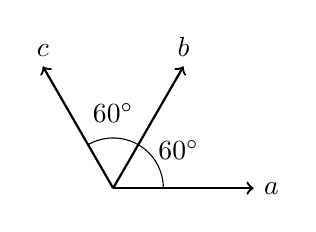
\begin{tikzpicture}[scale=0.85]
	\draw[->,thick] (0,0) -- (0:2.1) node[right] {$a$};
	\draw[->,thick] (0,0) -- (60:2.1) node[above] {$b$};
	\draw[->,thick] (0,0) -- (120:2.1) node[above] {$c$};
	\draw (0:0.75) arc (0:60:0.75);
	\draw (60:0.75) arc (60:120:0.75);
	\node at (30:1.13) {$60^\circ$};
	\node at (90:1.13) {$60^\circ$};
\end{tikzpicture}
\end{center}
\end{frame}


\begin{frame}{Violación de la desigualdad de Bell}{}
Utilizando la Ecuación \ref{eq:correlacion_MC},

\begin{align*}
	C_{\text{MC}}(a,b)=&-\cos60^\circ=-\frac{1}{2},
	\\
	C_{\text{MC}}(a,c)=&-\cos120^\circ=\frac{1}{2},
	\\
	C_{\text{MC}}(b,c)=&-\cos60^\circ=-\frac{1}{2}.
\end{align*}

Para satisfacer la Ecuación \ref{eq:des_bell}, tendría que cumplirse
$$ \left|-\frac{1}{2}-\frac{1}{2}\right|\leq 1-\frac{1}{2}. $$
\begin{block}{Violación de la desigualdad de Bell}
	$$ 1\not\leq\frac{1}{2}. $$
\end{block}
\end{frame}